\documentclass[11pt]{article}

\usepackage[utf8]{inputenc}
\usepackage[T1]{fontenc}
\usepackage{lmodern}
\usepackage[spanish, es-noshorthands, es-nodecimaldot, es-tabla]{babel}
\usepackage[margin=2.5cm]{geometry}
\usepackage{amsmath, amssymb, amsthm}
\usepackage{graphicx}
\usepackage{subcaption}
\usepackage{tabularx}
\usepackage{booktabs}
\usepackage{float}
\usepackage{algorithm}
\usepackage{algpseudocode}
\usepackage[hidelinks]{hyperref}

% babel-spanish redefine \% para anadirle un espacio fino, y eso choca con
% las unidades de pegamento cuando aparece en tablas o cerca de modo
% matematico. Se restaura el caracter simple.
\AtBeginDocument{\DeclareRobustCommand{\%}{\char37}}

\graphicspath{{../figuras/}}

\newtheorem{teorema}{Teorema}
\newtheorem{lema}{Lema}
\newtheorem{definicion}{Definición}
\newcolumntype{L}{>{\raggedright\arraybackslash}X}

% Pseudocódigo en español
\floatname{algorithm}{Algoritmo}
\algrenewcommand\algorithmicrequire{\textbf{Entrada:}}
\algrenewcommand\algorithmicensure{\textbf{Salida:}}
\algrenewcommand\algorithmicfor{\textbf{para}}
\algrenewcommand\algorithmicdo{\textbf{hacer}}
\algrenewcommand\algorithmicend{\textbf{fin}}
\algrenewcommand\algorithmicreturn{\textbf{devolver}}
\algrenewcommand\algorithmicwhile{\textbf{mientras}}
\algrenewcommand\algorithmicif{\textbf{si}}
\algrenewcommand\algorithmicelse{\textbf{si no}}
\algrenewcommand\algorithmicthen{\textbf{entonces}}

\title{Tarea 2: Números Pseudoaleatorios y Métodos de Monte Carlo\
       \large Curso Libre de Configuración 2: Análisis de Datos}
\author{Herman Andrés Echeverría Rojas\
        \small Facultad de Ingeniería, Universidad del Istmo de Guatemala}
\date{\today}

\begin{document}
\maketitle

\begin{abstract}
\noindent
Este documento acompaña al repositorio
\url{https://github.com/HermanEcheverria/numeros-pseudoaleatorios-montecarlo}.
Todas las figuras y tablas que aparecen aquí son generadas por los scripts del
repositorio a partir de las semillas registradas en \texttt{semillas.py}: no hay
ningún número transcrito a mano. Cualquiera puede clonar el repositorio,
ejecutar los scripts y obtener exactamente estos resultados.
\end{abstract}

\tableofcontents
\newpage

\part{Generadores de números pseudoaleatorios}

\section{Fundamento común}
\label{sec:fundamento}

Los cinco algoritmos que pide el enunciado (LCG, cuadrados medios, Mersenne
Twister, Blum Blum Shub y RANDU) parecen muy distintos entre sí, pero comparten
el mismo esqueleto. Conviene aislarlo una sola vez: de ahí salen dos resultados
—la periodicidad inevitable y la estructura de red— que después se aplican a
cada generador en particular.

\subsection{Qué es, formalmente, un generador pseudoaleatorio}

\begin{definicion}[Generador pseudoaleatorio]
\label{def:prng}
Un \emph{generador de números pseudoaleatorios} es una cuádrupla
$(\mathcal{S}, g, h, x_0)$ donde
\begin{itemize}
  \item $\mathcal{S}$ es un conjunto \textbf{finito} de estados,
  \item $g : \mathcal{S} \to \mathcal{S}$ es la \emph{función de transición},
  \item $h : \mathcal{S} \to [0,1)$ es la \emph{función de salida}, y
  \item $x_0 \in \mathcal{S}$ es la \emph{semilla}.
\end{itemize}
El generador produce la sucesión de estados $x_{n+1} = g(x_n)$ y la sucesión de
salidas $u_n = h(x_n)$.
\end{definicion}

Las tres piezas se reparten así en los algoritmos de esta tarea:

\begin{table}[H]
\centering
\small
\begin{tabularx}{\textwidth}{l L L L}
\toprule
Algoritmo & Estado $\mathcal{S}$ & Transición $g$ & Salida $h$ \\
\midrule
LCG / RANDU & $\{0,\dots,m-1\}$ & $x \mapsto (ax+c) \bmod m$ & $x/m$ \\
Cuadrados medios & enteros de $2k$ dígitos & dígitos centrales de $x^2$ & $x/10^{k}$ \\
Blum Blum Shub & $\mathbb{Z}_M^{*}$ & $x \mapsto x^2 \bmod M$ & bits bajos de $x$ \\
Mersenne Twister & $(\mathbb{Z}_2^{32})^{624}$ & torcedura lineal sobre $\mathbb{F}_2$ & templado de una palabra \\
\bottomrule
\end{tabularx}
\caption{Los cuatro esquemas bajo la misma estructura de la
Definición~\ref{def:prng}.}
\label{tab:esqueleto}
\end{table}

Dos consecuencias se leen directamente de la definición, antes de programar nada:

\paragraph{Determinismo.} Como $g$ es una función y $x_0$ está fijo, toda la
sucesión queda determinada por la semilla. Dos ejecuciones con la misma semilla
producen \emph{exactamente} la misma secuencia. Esto no es un defecto sino el
requisito de reproducibilidad que exige el enunciado; por eso cada generador de
este trabajo recibe su semilla como argumento explícito.

\paragraph{Ausencia de azar genuino.} La sucesión $(u_n)$ no es aleatoria en
ningún sentido probabilístico: es una sucesión fija. Lo único que se puede
pedir es que \emph{sea indistinguible} de una muestra i.i.d.\ $\mathrm{Unif}(0,1)$
frente a una batería de pruebas estadísticas dada. Esta sección se ocupa de la
parte determinista; las pruebas de hipótesis, de la otra.

\subsection{Toda sucesión pseudoaleatoria es periódica}

\begin{teorema}[Periodicidad eventual]
\label{teo:periodicidad}
Sea $(\mathcal{S}, g, h, x_0)$ un generador pseudoaleatorio con
$|\mathcal{S}| = N < \infty$. Entonces existen enteros
$\lambda \ge 0$ (la \emph{cola}) y $\rho \ge 1$ (el \emph{período}) tales que
\[
  x_{n+\rho} = x_n \qquad \text{para todo } n \ge \lambda,
\]
y además $\lambda + \rho \le N$.
\end{teorema}

\begin{proof}
Considérense los $N+1$ estados $x_0, x_1, \dots, x_N$. Todos pertenecen a
$\mathcal{S}$, que tiene solo $N$ elementos. Por el principio del palomar, dos
de ellos coinciden: existen índices $0 \le i < j \le N$ con $x_i = x_j$.

Sea $\rho = j - i \ge 1$. Como $x_{n+1}$ depende \emph{únicamente} de $x_n$,
aplicar $g$ a ambos lados de $x_i = x_j$ da $x_{i+1} = x_{j+1}$, y por inducción
$x_{i+k} = x_{j+k} = x_{i+k+\rho}$ para todo $k \ge 0$. Tomando
$\lambda = i$ se obtiene $x_{n+\rho} = x_n$ para todo $n \ge \lambda$.
Finalmente $\lambda + \rho = i + (j-i) = j \le N$.
\end{proof}

La demostración es corta pero dice tres cosas que importan en todo el trabajo:

\begin{enumerate}
  \item \textbf{El período nunca supera el número de estados}, $\rho \le N$.
        Aumentar el período obliga a agrandar el espacio de estados: es
        exactamente lo que hace el Mersenne Twister al guardar $624$ palabras de
        $32$ bits en lugar de un solo entero, alcanzando $\rho = 2^{19937}-1$.
  \item \textbf{Puede haber una cola $\lambda > 0$}: estados iniciales que nunca
        se vuelven a visitar. Esto ocurre cuando $g$ no es inyectiva, que es
        justamente el caso de los cuadrados medios. Si $g$ \emph{sí} es
        biyectiva —como en un LCG con $\gcd(a,m)=1$— entonces $\lambda = 0$ y la
        sucesión es puramente periódica desde el inicio.
  \item \textbf{La periodicidad es estructural, no un defecto de implementación.}
        Ningún algoritmo determinista sobre memoria finita puede evitarla. Lo
        único negociable es que $\rho$ sea tan grande que no se alcance en la
        práctica.
\end{enumerate}

\subsection{El generador congruencial lineal como caso de estudio}
\label{sec:fundamento-lcg}

El LCG es el más simple de los cinco y el único cuyo comportamiento se puede
caracterizar por completo con álgebra elemental. Por eso se deriva aquí: RANDU
resultará ser un caso particular suyo, y los defectos que se demuestren para la
familia se heredan automáticamente.

La recurrencia es
\begin{equation}
  x_{n+1} = (a\,x_n + c) \bmod m,
  \qquad n = 0, 1, 2, \dots
  \label{eq:lcg}
\end{equation}
con \emph{módulo} $m > 1$, \emph{multiplicador} $0 < a < m$, \emph{incremento}
$0 \le c < m$ y semilla $0 \le x_0 < m$. Si $c = 0$ el generador se llama
\emph{multiplicativo} (o de Lehmer); si $c \neq 0$, \emph{mixto}.

\subsubsection{Forma cerrada}

\begin{lema}[Forma cerrada del LCG]
\label{lema:forma-cerrada}
Para todo $n \ge 0$,
\begin{equation}
  x_n \equiv a^n x_0 + c \sum_{k=0}^{n-1} a^k \pmod{m}.
  \label{eq:forma-cerrada}
\end{equation}
\end{lema}

\begin{proof}
Por inducción sobre $n$.

\emph{Base.} Para $n = 0$ la suma es vacía (vale $0$) y el enunciado se reduce a
$x_0 \equiv a^0 x_0 = x_0$, que es cierto.

\emph{Paso inductivo.} Supóngase \eqref{eq:forma-cerrada} válida para $n$.
Aplicando la recurrencia \eqref{eq:lcg} y la hipótesis de inducción:
\begin{align*}
  x_{n+1} &\equiv a\,x_n + c
   \equiv a\left(a^n x_0 + c \sum_{k=0}^{n-1} a^k\right) + c \\
  &\equiv a^{n+1} x_0 + c \sum_{k=0}^{n-1} a^{k+1} + c
   \equiv a^{n+1} x_0 + c \sum_{k=1}^{n} a^{k} + c \\
  &\equiv a^{n+1} x_0 + c \sum_{k=0}^{n} a^{k} \pmod{m},
\end{align*}
donde el último paso absorbe el término $c = c\,a^0$ dentro de la suma. Esto es
\eqref{eq:forma-cerrada} para $n+1$.
\end{proof}

El Lema~\ref{lema:forma-cerrada} tiene una lectura incómoda: $x_n$ es una
función \emph{explícita y barata} de $n$. No hace falta iterar para saltar a
cualquier punto de la sucesión, y —lo que es peor para cualquier uso
criptográfico— basta observar unas pocas salidas consecutivas para plantear un
sistema y recuperar $(a, c, m)$. Ningún LCG es seguro, y la razón es esta
fórmula, no una debilidad de implementación.

\subsubsection{Período: el teorema de Hull--Dobell}

Por el Teorema~\ref{teo:periodicidad} el período cumple $\rho \le m$. La
pregunta natural es cuándo se alcanza la igualdad.

\begin{teorema}[Hull--Dobell, 1962 \cite{hulldobell}]
\label{teo:hull-dobell}
Un LCG mixto \eqref{eq:lcg} tiene período completo $\rho = m$ para
\textbf{toda} semilla $x_0$ si y solo si se cumplen las tres condiciones:
\begin{enumerate}
  \item $\gcd(c, m) = 1$;
  \item $a - 1$ es divisible por todo factor primo $q$ de $m$;
  \item si $4 \mid m$, entonces $4 \mid (a-1)$.
\end{enumerate}
\end{teorema}

\paragraph{Corolario para módulos potencia de dos.} Si $m = 2^k$ con $k \ge 2$,
el único factor primo de $m$ es $2$ y $4 \mid m$, de modo que las tres
condiciones colapsan en dos reglas verificables de un vistazo:
\begin{equation}
  c \text{ impar}
  \qquad\text{y}\qquad
  a \equiv 1 \pmod 4 .
  \label{eq:hd-potencia2}
\end{equation}
En efecto, $\gcd(c, 2^k) = 1 \iff c$ es impar; la condición (2) pide
$2 \mid (a-1)$ y la (3) pide $4 \mid (a-1)$, de las cuales la segunda implica la
primera. Este corolario explica de entrada por qué RANDU \emph{no} alcanza
período completo: al tener $c = 0$ falla la condición (1) desde el primer paso.

\subsubsection{Los casos degenerados}
\label{sec:degenerados}

Antes de programar conviene identificar qué elecciones de parámetros rompen el
generador, porque son las que la implementación debe rechazar explícitamente.

\paragraph{$a = 0$.} La recurrencia se vuelve $x_{n+1} = c \bmod m$ para todo
$n$: la sucesión es la constante $c/m$ desde el primer término. Período
$\rho = 1$.

\paragraph{$c = 0$ y $x_0 = 0$.} El cero es punto fijo de la recurrencia
multiplicativa, pues $g(0) = (a \cdot 0) \bmod m = 0$. Toda la sucesión es
idénticamente cero. Este caso es especialmente traicionero porque no lanza
ningún error: produce diez mil ceros que pasan desapercibidos si uno no mira el
histograma.

\paragraph{$a = 1$.} La recurrencia se reduce a $x_n = (x_0 + nc) \bmod m$, una
progresión aritmética. Tiene período completo si $\gcd(c,m)=1$, y sin embargo
las salidas son una rampa perfectamente predecible. Es el contraejemplo que
demuestra que \textbf{período completo no implica calidad}: Hull--Dobell es
necesario pero muy lejos de suficiente.

\subsection{Estructura de red: por qué las $k$-tuplas caen en hiperplanos}
\label{sec:red}

El defecto más serio de la familia LCG no lo detecta ninguna prueba
unidimensional. Aparece al mirar las salidas de $k$ en $k$.

\begin{teorema}[Estructura de red \cite{marsaglia}]
\label{teo:red}
Sea un LCG con parámetros $(a, c, m)$ y sea $k \ge 2$. Para todo vector de
enteros $\mathbf{h} = (h_0, h_1, \dots, h_{k-1})$ que satisfaga
\begin{equation}
  h_0 + h_1 a + h_2 a^2 + \dots + h_{k-1} a^{k-1} \equiv 0 \pmod{m},
  \label{eq:condicion-h}
\end{equation}
los puntos $\mathbf{u}_n = (u_n, u_{n+1}, \dots, u_{n+k-1})$ del cubo $[0,1)^k$
caen todos sobre una familia de hiperplanos paralelos, y el número de
hiperplanos efectivamente ocupados es a lo sumo $\sum_{i} |h_i|$.
\end{teorema}

\begin{proof}
Iterando el Lema~\ref{lema:forma-cerrada} desde $x_n$ en lugar de $x_0$,
\[
  x_{n+i} \equiv a^{i} x_n + c\, \sigma_i \pmod m ,
  \qquad
  \sigma_i := \sum_{j=0}^{i-1} a^{j} ,
\]
donde $\sigma_i$ \textbf{no depende de $n$}. Entonces
\[
  \sum_{i=0}^{k-1} h_i\, x_{n+i}
  \;\equiv\; x_n \underbrace{\sum_{i=0}^{k-1} h_i a^{i}}_{\equiv\, 0 \text{ por } \eqref{eq:condicion-h}}
  \;+\; c \underbrace{\sum_{i=0}^{k-1} h_i \sigma_i}_{=:\,K}
  \;\equiv\; cK \pmod m .
\]
El lado izquierdo es congruente módulo $m$ a una constante que no depende de
$n$, así que existe un entero $\ell_n$ con
$\sum_i h_i x_{n+i} = cK + \ell_n m$. Dividiendo entre $m$ y usando
$u_{n+i} = x_{n+i}/m$:
\begin{equation}
  \sum_{i=0}^{k-1} h_i\, u_{n+i} = \frac{cK}{m} + \ell_n .
  \label{eq:hiperplano}
\end{equation}
Para cada valor entero de $\ell_n$, la ecuación \eqref{eq:hiperplano} define un
hiperplano en $[0,1)^k$; al variar $n$ lo único que cambia es $\ell_n$, de modo
que todos los puntos viven en esa familia de hiperplanos paralelos. Como
$u_{n+i} \in [0,1)$, el lado izquierdo de \eqref{eq:hiperplano} está acotado en
un intervalo de longitud $\sum_i |h_i|$, luego $\ell_n$ solo puede tomar a lo
sumo $\sum_i |h_i|$ valores enteros distintos.
\end{proof}

Marsaglia \cite{marsaglia} demuestra además que \emph{siempre} existe un
$\mathbf{h}$ no trivial que cumple \eqref{eq:condicion-h} con coeficientes
pequeños, y que en consecuencia los puntos de cualquier LCG caen en no más de
$(k!\,m)^{1/k}$ hiperplanos. Para $k=3$ y $m = 2^{31}$ esa cota vale
\[
  (3! \cdot 2^{31})^{1/3} = (6 \cdot 2\,147\,483\,648)^{1/3} \approx 2344 ,
\]
que para efectos prácticos es inofensivo: $2344$ planos llenan el cubo de forma
razonablemente densa. El escándalo de RANDU —que se documenta en su propia
sección— es que se queda en \textbf{15}, dos órdenes de magnitud por debajo de
lo que la cota permitía.

\paragraph{Lectura operativa.} El Teorema~\ref{teo:red} explica por qué el
enunciado pide la \emph{prueba espectral visual} y no solo pruebas de hipótesis.
Las pruebas de uniformidad ($\chi^2$, Kolmogórov--Smirnov) miran una coordenada
a la vez; las de independencia serial (autocorrelación, rachas) miran
correlaciones lineales de a pares. Una relación exacta de tres términos como
\eqref{eq:condicion-h} es invisible para todas ellas y salta a la vista en el
diagrama de dispersión tridimensional. Es la diferencia entre no encontrar
evidencia y no haberla buscado donde estaba.

\subsection{Normalización}

Las salidas se obtienen dividiendo el estado entre el módulo, $u_n = x_n / m$.
Se divide entre $m$ y no entre $m-1$ porque el estado recorre
$\{0, 1, \dots, m-1\}$: el valor máximo posible es $(m-1)/m < 1$, que es
exactamente el soporte $[0,1)$ de la distribución $\mathrm{Unif}(0,1)$ estándar.
Dividir entre $m-1$ permitiría la salida $u = 1$, fuera del soporte, lo cual
rompe cualquier transformación posterior que use $\log(1-u)$ o la inversa de una
función de distribución acumulada.

Conviene tener presente que la salida es un valor de una rejilla discreta de
paso $1/m$, no un real del continuo. Ninguna implementación puede producir más
de $m$ valores distintos, y por eso una prueba de bondad de ajuste con más de
$m$ clases carecería de sentido.

\section{Los cinco generadores}
\label{sec:generadores}

Cada generador se presenta con su fundamento matemático, su pseudocódigo, y los
resultados de los incisos (a) y (b). Todas las semillas están registradas en
\texttt{semillas.py} y aparecen en el pie de cada figura.

\subsection{Generador congruencial lineal}

El fundamento está derivado en la Sección~\ref{sec:fundamento-lcg}: la
recurrencia \eqref{eq:lcg}, la forma cerrada del
Lema~\ref{lema:forma-cerrada} y el Teorema~\ref{teo:hull-dobell} de
Hull--Dobell.

\begin{algorithm}[H]
\caption{Generador congruencial lineal}
\begin{algorithmic}[1]
\Require $n$, semilla $x_0$, multiplicador $a$, incremento $c$, módulo $m$
\Ensure $n$ valores en $[0,1)$
\If{$a = 0$ \textbf{o} $a = 1$ \textbf{o} ($c = 0$ \textbf{y} $x_0 = 0$)}
  \State \textbf{error}: caso degenerado
\EndIf
\State $x \gets x_0$
\For{$i = 1$ \textbf{hasta} $n$}
  \State $x \gets (a\,x + c) \bmod m$
  \State $u_i \gets x / m$
\EndFor
\State \Return $(u_1,\dots,u_n)$
\end{algorithmic}
\end{algorithm}

Se usan los parámetros de \emph{Numerical Recipes}: $a = 1\,664\,525$,
$c = 1\,013\,904\,223$, $m = 2^{32}$. El corolario
\eqref{eq:hd-potencia2} se verifica de un vistazo: $c$ es impar y
$a - 1 = 1\,664\,524 = 4\cdot416\,131$, así que $a \equiv 1 \pmod 4$. El
período es completo, $2^{32}$.

\subsection{RANDU}

RANDU es el LCG con $a = 65\,539$, $c = 0$, $m = 2^{31}$. Al ser $c = 0$ falla
la primera condición de Hull--Dobell, y su período es el orden multiplicativo
de $a$ módulo $2^{31}$, que resulta ser $2^{29}$: desperdicia el 75\,\% de
los estados disponibles.

Su defecto nace de que $65\,539 = 2^{16}+3$. Elevando al cuadrado,
\[
  a^2 = (2^{16}+3)^2 = 2^{32} + 6\cdot 2^{16} + 9
      = 6\,(2^{16}+3) - 9 + 2^{32} = 6a - 9 + 2^{32},
\]
y como $2^{32} \equiv 0 \pmod{2^{31}}$, queda $a^2 \equiv 6a - 9$. Multiplicando
por $x_n$ se obtiene la identidad exacta
\begin{equation}
  x_{n+2} = 6\,x_{n+1} - 9\,x_n \pmod{2^{31}} .
  \label{eq:identidad-randu}
\end{equation}
Esta es la condición \eqref{eq:condicion-h} del Teorema~\ref{teo:red} con
$\mathbf{h} = (9,-6,1)$, y de ella salen los planos de la
Sección~\ref{sec:espectral}.

\paragraph{Verificación numérica.} La identidad \eqref{eq:identidad-randu} se
comprobó sobre los estados enteros (no normalizados, para que el redondeo de
punto flotante no la contamine) de una secuencia de $10\,000$ valores: se
cumple en las \textbf{9\,998} ternas, sin una sola excepción.

\paragraph{Sensibilidad a la semilla.} Como $c = 0$, se tiene
$x_n = a^n x_0 \bmod m$. Si la semilla es $x_0 = 2^s\cdot(\text{impar})$, el
factor $2^s$ sale de la recurrencia y el generador se comporta como si el
módulo fuera $2^{31-s}$: el período se parte a la mitad con cada factor 2.

\begin{table}[H]
\centering\small
\begin{tabular}{rrr}
\toprule
Semilla & Período & Salidas distintas de 64 \\
\midrule
$1$      & $536\,870\,912 = 2^{29}$ & 64 \\
$2$      & $268\,435\,456$ & 64 \\
$2^{16}$ & $8\,192$ & 64 \\
$2^{28}$ & $2$ & 2 \\
$2^{30}$ & $\mathbf{1}$ & $\mathbf{1}$ \\
\bottomrule
\end{tabular}
\caption{Degradación del período de RANDU según los factores de 2 de la
semilla.}
\label{tab:randu-semillas}
\end{table}

El caso extremo es contundente: con semilla $2^{30} = 1\,073\,741\,824$,
\textbf{RANDU devuelve $0.5$ para siempre}. La razón cabe en una línea: como
$65\,539$ es impar, $65\,539 \cdot 2^{30} \bmod 2^{31} = 2^{30}$, así que la
semilla es un punto fijo. Un generador anunciado con período $2^{29}$ entrega
una constante, y ninguna prueba de uniformidad avisa, porque el histograma es
una sola barra. Por eso la semilla usada en este trabajo es impar y
suficientemente grande para que $a\,x_0$ supere el módulo desde el primer paso.

\subsection{Método de los cuadrados medios}

Propuesto por von Neumann en 1949. El estado es un entero de $k$ dígitos (con
$k$ par); se eleva al cuadrado, se rellena con ceros a la izquierda hasta $2k$
posiciones y se extraen los $k$ dígitos centrales.

\begin{algorithm}[H]
\caption{Cuadrados medios (von Neumann)}
\begin{algorithmic}[1]
\Require $n$, semilla $x_0$ de $k$ dígitos, $k$ par
\Ensure $n$ valores en $[0,1)$
\State $x \gets x_0$
\For{$i = 1$ \textbf{hasta} $n$}
  \State $s \gets$ cadena de $x^2$ rellenada con ceros a la izquierda hasta $2k$ dígitos
  \State $x \gets$ entero formado por los dígitos $s_{k/2+1}, \dots, s_{k/2+k}$
  \State $u_i \gets x / 10^{k}$
\EndFor
\State \Return $(u_1,\dots,u_n)$
\end{algorithmic}
\end{algorithm}

\paragraph{No hay teoría de período.} A diferencia del LCG, este método carece
de un resultado tipo Hull--Dobell: el período depende de la semilla de un modo
que solo se conoce midiéndolo. La implementación se validó primero contra dos
secuencias publicadas: la de von Neumann con $k=2$ y semilla 43
($43 \to 84 \to 05 \to 02 \to 00$, la «trampa del cero» en cuatro pasos) y el
ciclo corto de $k=4$ ($6100 \to 2100 \to 4100 \to 8100 \to 6100$). Ambas se
reproducen exactamente.

\paragraph{Censo exhaustivo.} Con $k=4$ hay solo $10\,000$ semillas posibles,
así que el período no se estima: se recorre el espacio completo.

\begin{table}[H]
\centering\small
\begin{tabular}{rrr}
\toprule
Período & Semillas & Porcentaje \\
\midrule
1 & 2,263 & 22.6\% \\
4 & 7,737 & 77.4\% \\
\bottomrule
\end{tabular}

\caption{Período de las $10\,000$ semillas de 4 dígitos. Barrido exhaustivo.}
\label{tab:cm-censo}
\end{table}

\textbf{El período máximo sobre todas las semillas posibles es 4.} No existe
una sola semilla de 4 dígitos que produzca algo mejor. Las $2\,263$ de período
1 caen en cinco puntos fijos distintos: el $0$ (que absorbe $1\,968$ semillas y
es el «mecanismo cero» clásico), $2500$ (130), $100$ (104), $7600$ (60) y
$3792$, que es un caso curioso: $3792^2 = 14\,379\,264$, cuyos cuatro dígitos
centrales son $3792$, y ninguna otra semilla llega a él.

Para producir $10\,000$ valores sin repetición hace falta subir a 12 dígitos.
Con la semilla registrada, la órbita tiene una \textbf{cola de $326\,565$
estados} antes de entrar en un \textbf{ciclo de $2\,500$}. Esa cola es la
$\lambda > 0$ del Teorema~\ref{teo:periodicidad}: existe porque la función de
transición no es inyectiva, cosa imposible en un LCG con $\gcd(a,m)=1$.

\subsection{Mersenne Twister (MT19937)}

Recurrencia lineal sobre $\mathbb{F}_2$ con 624 palabras de 32 bits de estado y
período $2^{19937}-1$, un primo de Mersenne. Tiene tres etapas.

\begin{algorithm}[H]
\caption{MT19937}
\begin{algorithmic}[1]
\Require semilla $s$ de 32 bits
\Statex \textbf{Inicialización}
\State $mt[0] \gets s$
\For{$i = 1$ \textbf{hasta} $623$}
  \State $mt[i] \gets \bigl(1\,812\,433\,253 \cdot (mt[i-1] \oplus (mt[i-1] \gg 30)) + i\bigr) \bmod 2^{32}$
\EndFor
\Statex \textbf{Torcedura} (cuando se agotan las 624 palabras)
\For{$i = 0$ \textbf{hasta} $623$}
  \State $x \gets (mt[i] \wedge \texttt{0x80000000}) \vee (mt[(i{+}1)\bmod 624] \wedge \texttt{0x7FFFFFFF})$
  \State $x_A \gets x \gg 1$; \textbf{si} $x$ es impar \textbf{entonces} $x_A \gets x_A \oplus \texttt{0x9908B0DF}$
  \State $mt[i] \gets mt[(i{+}397)\bmod 624] \oplus x_A$
\EndFor
\Statex \textbf{Templado} (al emitir cada palabra)
\State $y \gets mt[\text{índice}]$
\State $y \gets y \oplus (y \gg 11)$
\State $y \gets y \oplus ((y \ll 7) \wedge \texttt{0x9D2C5680})$
\State $y \gets y \oplus ((y \ll 15) \wedge \texttt{0xEFC60000})$
\State $y \gets y \oplus (y \gg 18)$
\State \Return $y / 2^{32}$
\end{algorithmic}
\end{algorithm}

\paragraph{Verificación.} La especificación publica la salida para la semilla
de referencia $5489$. La implementación la reproduce exactamente:

\begin{table}[H]
\centering\small
\begin{tabular}{rrrc}
\toprule
$i$ & Implementación & Especificación & Coincide \\
\midrule
1 & 3499211612 & 3499211612 & Sí \\
2 & 581869302 & 581869302 & Sí \\
3 & 3890346734 & 3890346734 & Sí \\
4 & 3586334585 & 3586334585 & Sí \\
5 & 545404204 & 545404204 & Sí \\
\bottomrule
\end{tabular}

\caption{Primeras palabras de 32 bits con semilla $5489$, contra el vector de
referencia de la especificación (OEIS A221557).}
\label{tab:mt-verificacion}
\end{table}

Las diez coinciden, y además coinciden con las palabras crudas de
\texttt{numpy.random.RandomState(5489)}. Dos fuentes independientes.

\paragraph{Equidistribución y seguridad.} MT19937 está equidistribuido en 623
dimensiones: sus $k$-tuplas llenan el hipercubo uniformemente hasta $k=623$.
Ese es el contraste exacto con RANDU, que falla ya en $k=3$. Sin embargo
\textbf{no es criptográficamente seguro}: el templado es una transformación
invertible, así que observando 624 salidas consecutivas se reconstruye el
estado interno y se predice todo el resto.

\subsection{Blum Blum Shub}

Recurrencia $x_{n+1} = x_n^2 \bmod M$ con $M = pq$ y $p,q$ primos de Blum
($\equiv 3 \bmod 4$).

\begin{algorithm}[H]
\caption{Blum Blum Shub}
\begin{algorithmic}[1]
\Require $n$, semilla $s$ coprima con $M$, primos de Blum $p,q$
\State $M \gets p\,q$; \quad $k \gets \lfloor \log_2 \log_2 M \rfloor$
\State $x \gets s^2 \bmod M$ \Comment{garantiza que $x$ sea residuo cuadrático}
\While{falten salidas}
  \State $x \gets x^2 \bmod M$
  \State acumular los $k$ bits menos significativos de $x$
  \State \textbf{si} hay 32 bits acumulados \textbf{entonces} emitir su valor dividido entre $2^{32}$
\EndWhile
\end{algorithmic}
\end{algorithm}

\begin{table}[H]
\centering\small
\begin{tabular}{lc}
\toprule
Condición & Se cumple \\
\midrule
p = 2147483783 es primo & Sí \\
q = 2148484187 es primo & Sí \\
p = 3 (mod 4): p mod 4 = 3 & Sí \\
q = 3 (mod 4): q mod 4 = 3 & Sí \\
p es seguro: (p-1)/2 = 1073741891 primo & Sí \\
q es seguro: (q-1)/2 = 1074242093 primo & Sí \\
gcd((p-3)/2, (q-3)/2) = 2 es pequeño & Sí \\
\bottomrule
\end{tabular}

\caption{Condiciones verificadas sobre los primos elegidos.}
\label{tab:bbs-condiciones}
\end{table}

\paragraph{El período.} Como $x_n = x_0^{2^n} \bmod M$, la sucesión se repite
cuando $2^n$ recupera su valor módulo el orden de $x_0$. El cálculo tiene dos
trampas. Primero, el orden \emph{no} se toma módulo $\lambda(M) = 2p'q'$, que
es par y donde 2 ni siquiera es invertible; como $x_0$ es residuo cuadrático,
su orden divide $\lambda(M)/2 = p'q'$, que es impar. Segundo, el orden de 2
módulo $p'q'$ divide el exponente del grupo de unidades, $\mathrm{lcm}(p'-1,
q'-1)$, y no $p'q'$. Con los primos elegidos el período resulta
$2\,353\,997\,416\,697\,212 \approx 2^{51}$.

La fórmula se verificó contra el período observado iterando, con primos seguros
pequeños: $(p,q) = (11,23)$ da 20 predicho y 20 observado; $(23,47)$ da 110 y
110; $(47,59)$ da 308 y 308.

\paragraph{Seguridad y costo.} Es el único de los cinco criptográficamente
seguro: distinguir su salida de una secuencia aleatoria es tan difícil como
resolver el problema de la residuosidad cuadrática módulo $M$, que se apoya en
la dificultad de factorizar $M$. La garantía exige emitir a lo sumo
$\lfloor\log_2\log_2 M\rfloor = 5$ bits por estado; emitir el estado completo
la destruiría. De ahí que necesite varias exponenciaciones modulares por
número, contra una multiplicación del LCG, y que sea diez veces más lento.

\subsection{Resultados de los incisos (a) y (b)}

\begin{figure}[H]
\centering
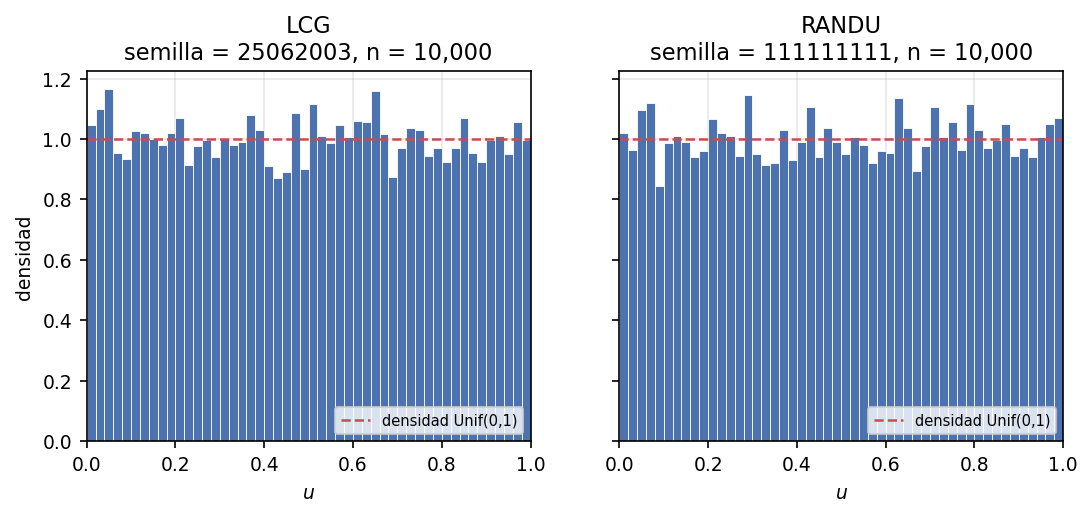
\includegraphics[width=\textwidth]{hist_lcg_randu.png}
\\[0.6em]
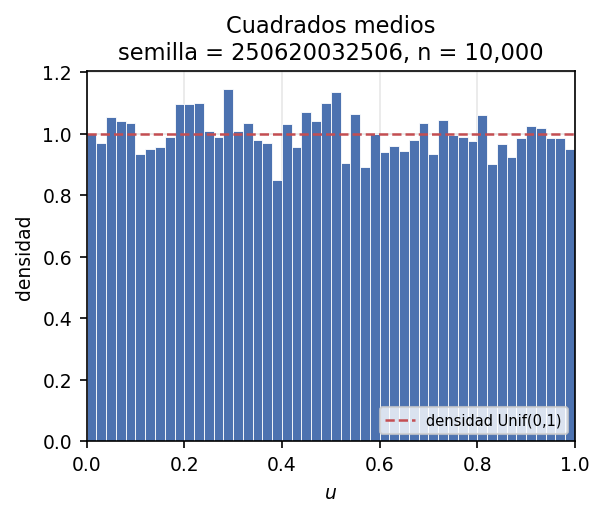
\includegraphics[width=0.32\textwidth]{hist_cuadrados_medios.png}
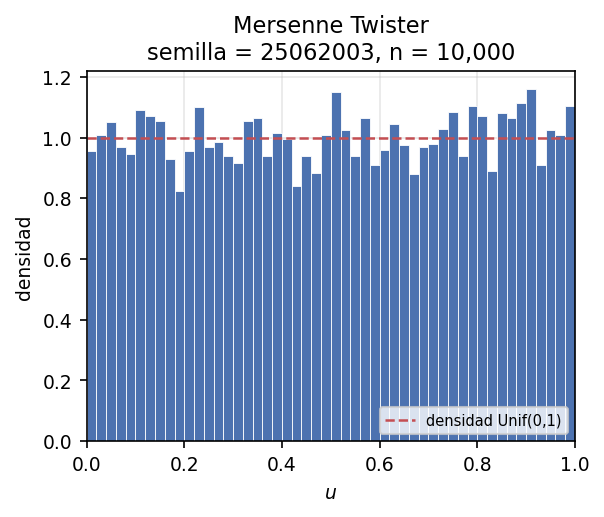
\includegraphics[width=0.32\textwidth]{hist_mersenne.png}
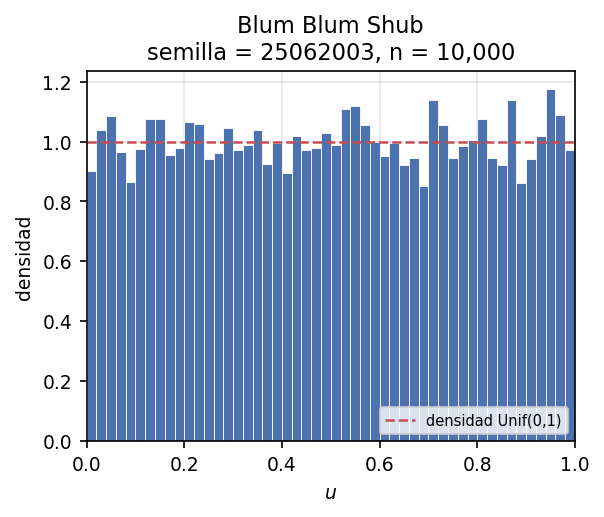
\includegraphics[width=0.32\textwidth]{hist_bbs.png}
\caption{Histogramas normalizados de los cinco generadores, $n = 10\,000$, con
la densidad teórica $\mathrm{Unif}(0,1)$ superpuesta.}
\label{fig:histogramas}
\end{figure}

\begin{table}[H]
\centering\small
\begin{tabular}{llrrl}
\toprule
Generador & Prueba & Estadístico & $p$-valor & Decisión ($\alpha=0.05$) \\
\midrule
LCG & $\chi^2$ & 44.2400 & 0.6662 & No se rechaza \\
LCG & K--S & 0.0075 & 0.6306 & No se rechaza \\
LCG & Autocorr. & 0.0102 & 0.3087 & No se rechaza \\
LCG & Rachas & 4965.0000 & 0.4715 & No se rechaza \\
RANDU & $\chi^2$ & 42.6600 & 0.7265 & No se rechaza \\
RANDU & K--S & 0.0072 & 0.6732 & No se rechaza \\
RANDU & Autocorr. & -0.0210 & 0.0353 & Se rechaza \\
RANDU & Rachas & 5030.0000 & 0.5619 & No se rechaza \\
\bottomrule
\end{tabular}

\caption{Pruebas de hipótesis para LCG y RANDU.}
\label{tab:pruebas-lcg}
\end{table}

\begin{table}[H]
\centering\small
\begin{minipage}{0.48\textwidth}\centering
\begin{tabular}{lrrl}
\toprule
Prueba & Estadístico & $p$-valor & Decisión ($\alpha=0.05$) \\
\midrule
$\chi^2$ & 38.9000 & 0.8489 & No se rechaza \\
K--S & 0.0109 & 0.1823 & No se rechaza \\
Autocorr. & 0.0076 & 0.4464 & No se rechaza \\
Rachas & 4964.0000 & 0.4593 & No se rechaza \\
\bottomrule
\end{tabular}
\\[0.3em]
\footnotesize Cuadrados medios
\end{minipage}
\begin{minipage}{0.48\textwidth}\centering
\begin{tabular}{lrrl}
\toprule
Prueba & Estadístico & $p$-valor & Decisión ($\alpha=0.05$) \\
\midrule
$\chi^2$ & 61.1500 & 0.1142 & No se rechaza \\
K--S & 0.0125 & 0.0853 & No se rechaza \\
Autocorr. & 0.0005 & 0.9599 & No se rechaza \\
Rachas & 5000.0000 & 0.9840 & No se rechaza \\
\bottomrule
\end{tabular}
\\[0.3em]
\footnotesize Mersenne Twister
\end{minipage}
\\[1em]
\begin{minipage}{\textwidth}\centering
\begin{tabular}{lrrl}
\toprule
Prueba & Estadístico & $p$-valor & Decisión ($\alpha=0.05$) \\
\midrule
$\chi^2$ & 55.4700 & 0.2440 & No se rechaza \\
K--S & 0.0062 & 0.8305 & No se rechaza \\
Autocorr. & 0.0129 & 0.1959 & No se rechaza \\
Rachas & 4979.0000 & 0.6599 & No se rechaza \\
\bottomrule
\end{tabular}
\\[0.3em]
\footnotesize Blum Blum Shub
\end{minipage}
\caption{Pruebas de hipótesis para los tres generadores restantes.}
\label{tab:pruebas-resto}
\end{table}

\paragraph{Interpretación.} Los cinco generadores pasan las cuatro pruebas.
Pasa el criptográficamente seguro y pasa el que tiene cinco puntos fijos y un
período máximo de 4 con cuatro dígitos. Pasa RANDU, que lleva dentro la
identidad exacta \eqref{eq:identidad-randu}.

Eso no es un defecto de las pruebas sino su alcance: $\chi^2$ y
Kolmogórov--Smirnov examinan una coordenada a la vez, y la autocorrelación de
retardo 1 y las rachas examinan relaciones entre pares consecutivos. Una
relación de tres términos es invisible para las cuatro. \textbf{Una batería de
pruebas certifica únicamente aquello que las pruebas miran.}

\subsection{Robustez sobre múltiples semillas}

Una sola corrida puede engañar en ambas direcciones. Con la semilla registrada,
RANDU \emph{rechaza} la prueba de autocorrelación con $p = 0.0353$, lo que
invitaría a concluir que esa prueba detectó su defecto. Para comprobarlo se
aplicó el esquema de dos niveles de NIST SP 800-22: la batería se repite sobre
$K = 100$ semillas y se analiza la distribución de los $p$-valores.

Las 100 semillas no pueden elegirse consecutivas. En un LCG de período completo
todas las semillas viven en el mismo ciclo, y dos semillas cercanas dan
secuencias que se solapan casi por completo. Se obtienen saltando exactamente
$10\,000$ posiciones mediante la forma cerrada del
Lema~\ref{lema:forma-cerrada}, lo que las deja disjuntas por construcción; el
salto se verificó contra iteración directa para los tres juegos de parámetros.

\begin{table}[H]
\centering\small
\begin{tabular}{llrrcrr}
\toprule
Generador & Prueba & Rechazos & Banda NIST & Dentro & $\chi^2$ unif. & $p$ \\
\midrule
LCG & $\chi^2$ & 3.0% & [0.0%, 11.5%] & Sí & 11.40 & 0.2493 \\
LCG & K--S & 4.0% & [0.0%, 11.5%] & Sí & 16.00 & 0.0669 \\
LCG & Autocorr. & 1.0% & [0.0%, 11.5%] & Sí & 12.40 & 0.1917 \\
LCG & Rachas & 4.0% & [0.0%, 11.5%] & Sí & 5.20 & 0.8165 \\
RANDU & $\chi^2$ & 3.0% & [0.0%, 11.5%] & Sí & 6.40 & 0.6993 \\
RANDU & K--S & 4.0% & [0.0%, 11.5%] & Sí & 10.60 & 0.3041 \\
RANDU & Autocorr. & 3.0% & [0.0%, 11.5%] & Sí & 11.00 & 0.2757 \\
RANDU & Rachas & 6.0% & [0.0%, 11.5%] & Sí & 13.40 & 0.1453 \\
\bottomrule
\end{tabular}

\caption{Tasa de rechazo sobre 100 semillas disjuntas y uniformidad de los
$p$-valores. La banda de NIST es $\alpha \pm 3\sqrt{\alpha(1-\alpha)/K}$.}
\label{tab:robustez}
\end{table}

\begin{figure}[H]
\centering
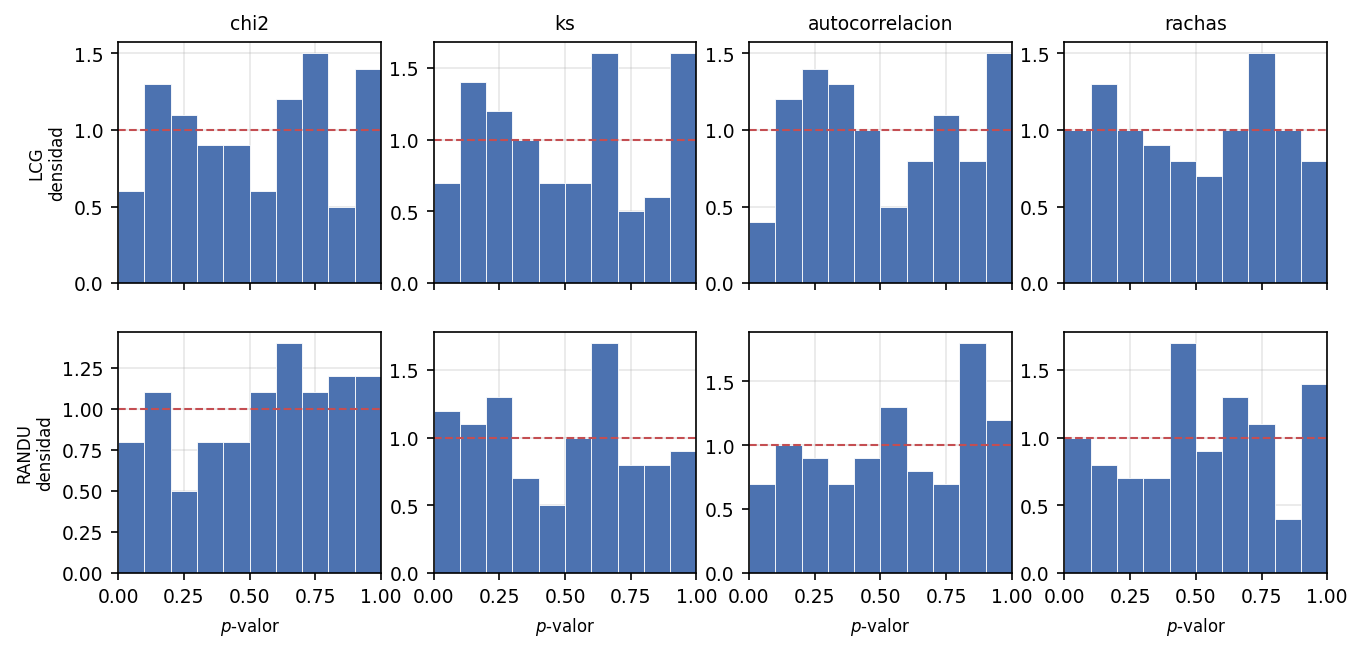
\includegraphics[width=\textwidth]{pvalores.png}
\caption{Distribución de los $p$-valores sobre 100 semillas. Bajo $H_0$ deben
ser $\mathrm{Unif}(0,1)$, es decir planos en 1.}
\label{fig:pvalores}
\end{figure}

La tasa de rechazo de RANDU en la prueba de autocorrelación es del $3\,\%$,
dentro de la banda: aquel rechazo aislado fue un \textbf{error de tipo I}, no
una detección. Las ocho tasas caen dentro de lo esperado y los ocho
histogramas son compatibles con la uniformidad. Con 800 $p$-valores en lugar de
8, la conclusión se sostiene mucho mejor: estas cuatro pruebas no encuentran
nada malo en RANDU.

\section{Prueba espectral}
\label{sec:espectral}

El Teorema~\ref{teo:red} predice que las ternas de un LCG caen en planos. Se
grafican las ternas consecutivas $(u_i,u_{i+1},u_{i+2})$ en el cubo $[0,1)^3$.

\paragraph{El ángulo de vista está derivado, no ajustado.} La cámara apunta en
la dirección $\mathbf{d} = (\cos e\cos a,\ \cos e \sin a,\ \sin e)$, donde $e$
es la elevación y $a$ el azimut. Los planos se ven de canto cuando se mira
\emph{paralelo} a ellos, es decir cuando $\mathbf{d}$ es perpendicular a la
normal: $\mathbf{d}\cdot\mathbf{h} = 0$ con $\mathbf{h} = (9,-6,1)$. Resolviendo
numéricamente se obtiene $e = 47^\circ$, $a = 62^\circ$, con residuo
$5\times10^{-5}$.

\begin{figure}[H]
\centering
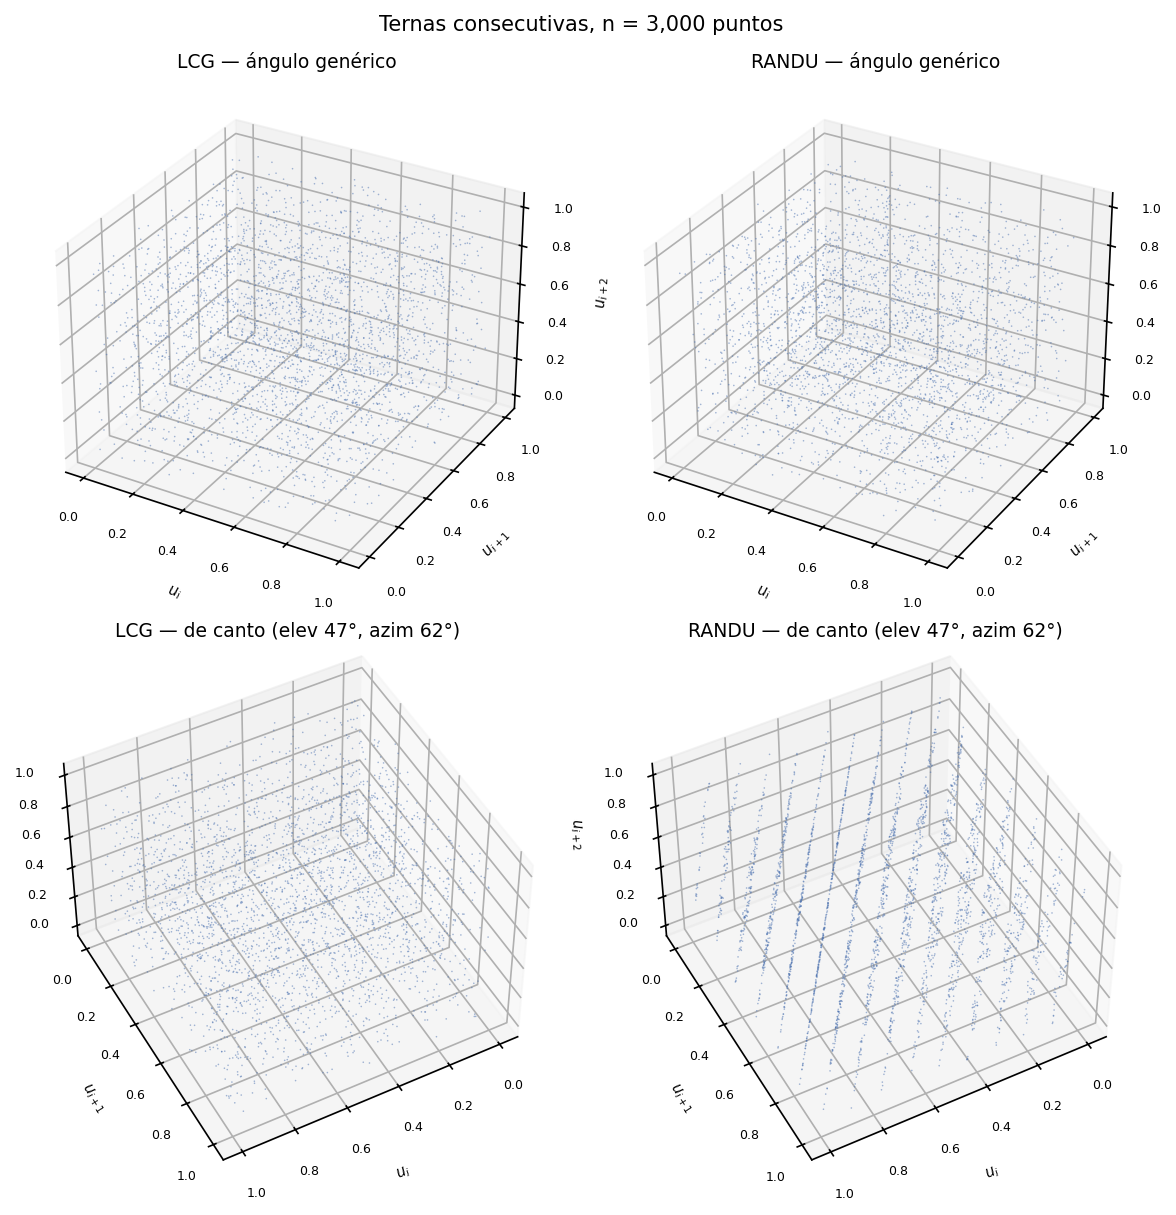
\includegraphics[width=0.92\textwidth]{espectral_3d.png}
\caption{Ternas consecutivas, $3\,000$ puntos. Arriba, el ángulo por defecto:
ambos generadores parecen ruido. Abajo, el ángulo derivado: RANDU colapsa en
líneas.}
\label{fig:espectral3d}
\end{figure}

La fila superior es tan importante como la inferior. Desde un ángulo genérico
RANDU y el LCG son indistinguibles a simple vista: el defecto solo aparece si
se mira desde la dirección correcta.

\paragraph{La demostración cuantitativa.} La gráfica convence; el conteo
demuestra. Para cada terna se calcula $k_i = 9u_i - 6u_{i+1} + u_{i+2}$, que
por \eqref{eq:identidad-randu} debe ser entero en RANDU.

\begin{figure}[H]
\centering
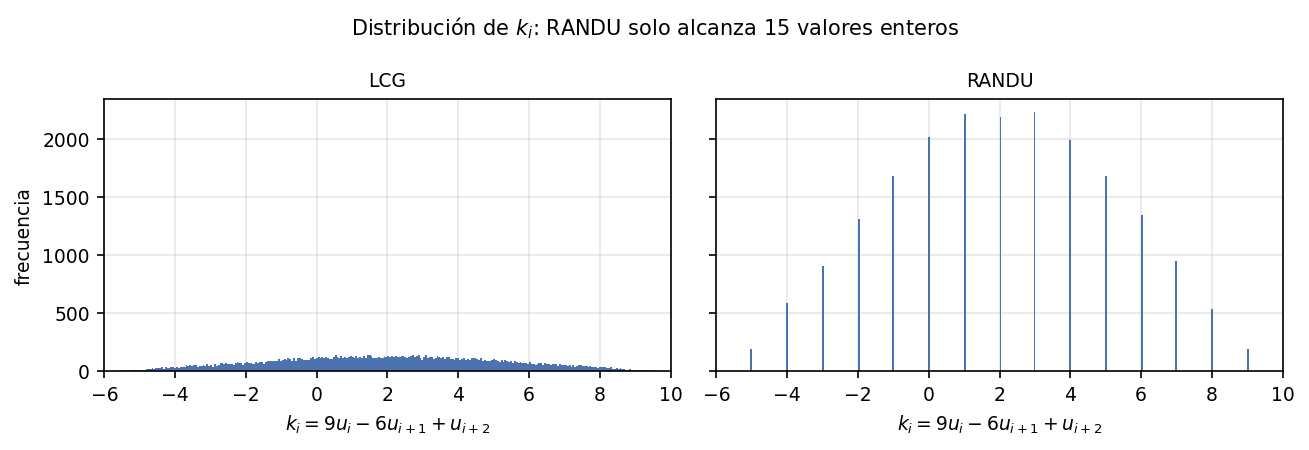
\includegraphics[width=\textwidth]{espectral_k.png}
\caption{Distribución de $k_i$ sobre $20\,000$ ternas.}
\label{fig:espectralk}
\end{figure}

\begin{table}[H]
\centering\small
\begin{tabular}{lrrr}
\toprule
Generador & Planos ocupados & Rango de $k_i$ & Desv. máx. al entero \\
\midrule
LCG & 0 & [-5.904, 9.790] & 5.0e-01 \\
RANDU & 15 & [-5.000, 9.000] & 0.0e+00 \\
\bottomrule
\end{tabular}

\caption{Conteo de planos ocupados.}
\label{tab:espectral}
\end{table}

RANDU toma exactamente \textbf{15} valores, $k \in \{-5,\dots,9\}$, con
desviación $0.00$ respecto al entero más cercano: la relación es algebraica,
no aproximada. El LCG de Numerical Recipes toma 0 valores enteros y su $k_i$ se
distribuye de forma continua.

El conteo coincide con la predicción del Teorema~\ref{teo:red}: como cada
$u\in[0,1)$, la combinación $9u_i-6u_{i+1}+u_{i+2}$ está acotada entre $-6$ y
$10$, así que solo caben los 15 enteros de $-5$ a $9$. Se predijeron 15 y se
observaron 15.

\paragraph{Relación con el período y la calidad.} RANDU tiene período
$2^{29} \approx 5.4\times10^8$: más de quinientos millones de valores antes de
repetirse. Y sus ternas ocupan 15 planos. Son propiedades
\textbf{independientes}: el período mide cuánto tarda la secuencia en repetirse
y la prueba espectral mide qué tan bien llena el espacio. Un generador puede
tardar una eternidad en repetirse y distribuir pésimo en tres dimensiones.

Peor aún, la cota de Marsaglia permitía hasta
$(3!\cdot 2^{31})^{1/3} \approx 2344$ planos, que habría sido inofensivo.
RANDU se queda en 15: unas 150 veces por debajo de su propio peor caso
permitido.

\section{Tabla comparativa}
\label{sec:comparativa}

\begin{table}[H]
\centering\footnotesize
\begin{tabular}{lrrlp{4cm}p{4cm}}
\toprule
Algoritmo & s / $10^6$ & Rel. & Período & Seguridad & Casos de uso \\
\midrule
LCG (Num. Recipes) & 0.15 & 1.0$\times$ & $2^{32}$ & Nula: la forma cerrada permite recuperar $(a,c,m)$ con pocas salidas. & Simulación sencilla, videojuegos, sistemas embebidos, \texttt{rand()} de C. \\
RANDU & 0.15 & 1.0$\times$ & $2^{29}$ & Nula, y además las ternas caen en 15 planos. & Ninguno. Solo interés histórico y didáctico. \\
Cuadrados medios & 0.29 & 1.9$\times$ & cola $326\,565$ + ciclo $2\,500$ & Nula. Degenera: cinco puntos fijos con 4 dígitos. & Ninguno. Obsoleto desde los años 50. \\
Mersenne Twister & 0.66 & 4.4$\times$ & $2^{19937}-1$ & Nula: con 624 salidas se reconstruye el estado. & Estándar de simulación. Motor de \texttt{random} de Python. \\
Blum Blum Shub & 1.47 & 9.8$\times$ & $\approx 2^{51}$ & \textbf{Criptográfica}: equivale a la residuosidad cuadrática módulo $M$. & Criptografía, donde la lentitud es aceptable. \\
\bottomrule
\end{tabular}

\caption{Comparación de los cinco generadores. Las velocidades están
cronometradas en esta máquina (mejor de tres corridas); los períodos son
derivados donde hay teoría y medidos donde no la hay.}
\label{tab:comparativa}
\end{table}

El orden de velocidad reproduce el costo algebraico de cada recurrencia. El LCG
y RANDU son idénticos en costo, como debe ser: RANDU \emph{es} un LCG. Los
cuadrados medios pagan la conversión a cadena de dígitos. MT19937 paga la
torcedura de 624 palabras. Y BBS es diez veces más lento que el LCG porque
necesita varias exponenciaciones modulares para producir un solo número, ya que
solo puede emitir 5 bits por estado.

\subsection{Comparación con \texttt{random} y \texttt{secrets}}
\label{sec:librerias}

Para el inciso (d) se eligió MT19937 por una razón concreta: \texttt{random} de
Python \emph{es} MT19937. Al tratarse del mismo algoritmo, cualquier diferencia
mide la implementación y no la calidad del generador.

\begin{table}[H]
\centering\small
\begin{tabular}{lrcrrrr}
\toprule
Fuente & s / $10^6$ & Reproducible & $\chi^2$ & K--S & Autocorr. & Rachas \\
\midrule
MT19937 (propio) & 0.61 & Sí & 0.1142 & 0.0853 & 0.9599 & 0.9840 \\
random (MT19937 de C) & 0.05 & Sí & 0.3267 & 0.8335 & 0.8447 & 0.8729 \\
secrets (SystemRandom) & 0.24 & \textbf{No} & 0.6728 & 0.2604 & 0.8060 & 0.7949 \\
\bottomrule
\end{tabular}

\caption{Comparación del MT19937 propio contra las librerías estándar.}
\label{tab:librerias}
\end{table}

La implementación propia es unas doce veces más lenta que \texttt{random}, y
eso no dice nada sobre el algoritmo: es Python interpretado contra C compilado.
El detalle revelador es que \texttt{secrets} resulta \emph{más rápido} que el
MT19937 propio pese a ser criptográficamente seguro. Tampoco es una ventaja
algorítmica: \texttt{secrets} delega en el generador del sistema operativo, que
también está en C. Lo caro no es la criptografía, es el bucle de Python.

La diferencia que sí es de diseño está en la reproducibilidad.
\texttt{secrets} no acepta semilla, y no por omisión sino a propósito: un
generador criptográfico predecible no sirve de nada. Eso lo vuelve inutilizable
para simulación reproducible, que es justamente lo que este trabajo exige.


\part{Métodos de Monte Carlo}

\section{Fundamento: el estimador y su error}
\label{sec:mc-fundamento}

Esta sección deriva los tres resultados que sostienen todo lo que sigue: que el
estimador de Monte Carlo es insesgado, que su error decae como $O(N^{-1/2})$
sin importar la dimensión, y cómo se construye su intervalo de confianza.

\subsection{La integral como valor esperado}

Sea $f$ integrable en $[a,b]$ y sea $I = \int_a^b f(x)\,dx$. Si
$U \sim \mathrm{Unif}(a,b)$, su densidad es $p(x) = 1/(b-a)$ sobre $[a,b]$ y
cero fuera. Entonces, por definición de valor esperado,
\begin{equation}
  \mathbb{E}[f(U)] = \int_a^b f(x)\, p(x)\, dx
  = \frac{1}{b-a}\int_a^b f(x)\,dx = \frac{I}{b-a},
  \label{eq:esperanza}
\end{equation}
de donde
\begin{equation}
  \boxed{\;I = (b-a)\,\mathbb{E}[f(U)]\;}
  \label{eq:integral-esperanza}
\end{equation}

El paso es puramente algebraico, pero cambia la naturaleza del problema:
calcular una integral pasa a ser \emph{estimar una media}. Y una media se
estima promediando muestras.

\subsection{El estimador es insesgado}

Sean $U_1, \dots, U_N$ independientes e idénticamente distribuidas
$\mathrm{Unif}(a,b)$, y defínase
\begin{equation}
  \hat I_N = \frac{b-a}{N}\sum_{i=1}^{N} f(U_i).
  \label{eq:estimador}
\end{equation}

\begin{teorema}[Insesgadez]
\label{teo:insesgado}
$\mathbb{E}[\hat I_N] = I$ para todo $N \ge 1$.
\end{teorema}

\begin{proof}
Por linealidad del valor esperado, que no requiere independencia:
\[
  \mathbb{E}[\hat I_N]
  = \frac{b-a}{N}\, \mathbb{E}\!\left[\sum_{i=1}^{N} f(U_i)\right]
  = \frac{b-a}{N} \sum_{i=1}^{N} \mathbb{E}[f(U_i)].
\]
Como todas las $U_i$ tienen la misma distribución, cada sumando vale lo mismo,
$\mathbb{E}[f(U_i)] = \mathbb{E}[f(U)] = I/(b-a)$ por \eqref{eq:esperanza}.
Hay $N$ sumandos iguales, así que
\[
  \mathbb{E}[\hat I_N] = \frac{b-a}{N} \cdot N \cdot \frac{I}{b-a} = I. \qedhere
\]
\end{proof}

Conviene subrayar qué \emph{no} dice el teorema. Insesgado significa que el
estimador acierta \emph{en promedio sobre infinitas repeticiones}, no que una
corrida particular esté cerca. Cuán cerca está una corrida es justamente lo que
mide la varianza.

\subsection{La varianza y la tasa $O(N^{-1/2})$}

\begin{teorema}[Varianza del estimador]
\label{teo:varianza}
Si $\sigma_f^2 := \mathrm{Var}(f(U)) < \infty$, entonces
\begin{equation}
  \mathrm{Var}(\hat I_N) = \frac{(b-a)^2 \sigma_f^2}{N},
  \qquad\text{y por lo tanto}\qquad
  \mathrm{EE}(\hat I_N) = \frac{(b-a)\,\sigma_f}{\sqrt{N}} .
  \label{eq:varianza}
\end{equation}
\end{teorema}

\begin{proof}
Aquí sí hace falta la independencia. Para variables independientes la varianza
de la suma es la suma de las varianzas, y $\mathrm{Var}(cX) = c^2\mathrm{Var}(X)$:
\[
  \mathrm{Var}(\hat I_N)
  = \left(\frac{b-a}{N}\right)^{\!2} \mathrm{Var}\!\left(\sum_{i=1}^{N} f(U_i)\right)
  = \frac{(b-a)^2}{N^2} \sum_{i=1}^{N} \mathrm{Var}(f(U_i))
  = \frac{(b-a)^2}{N^2} \cdot N\sigma_f^2 ,
\]
que se simplifica a \eqref{eq:varianza}. El error estándar es la raíz.
\end{proof}

El error estándar decae como $N^{-1/2}$. Es una tasa \textbf{lenta}: para
ganar un dígito decimal de precisión hay que multiplicar $N$ por cien. Pero
tiene una propiedad que la vuelve valiosa.

\paragraph{Por qué la tasa no depende de la dimensión.} Obsérvese qué entra en
la fórmula \eqref{eq:varianza}: solamente $N$ y $\sigma_f^2$. La dimensión
\emph{no aparece}. La razón es que la derivación nunca usó que $U$ fuera un
número real: solo usó que las $f(U_i)$ fueran independientes, idénticamente
distribuidas y de varianza finita. Si $U$ es un punto en $\mathbb{R}^d$, cada
$f(U_i)$ sigue siendo un \emph{escalar}, el promedio sigue siendo un promedio
de $N$ números, y el mismo cálculo se aplica palabra por palabra.

El contraste con los métodos determinísticos es lo que da valor a esto. Una
regla de cuadratura sobre una rejilla de $m$ puntos por eje necesita $m^d$
evaluaciones, y su error típico es $O(m^{-k}) = O(N^{-k/d})$ para un método de
orden $k$: la tasa \emph{se degrada} al crecer $d$. Monte Carlo mantiene
$N^{-1/2}$ para todo $d$. Existe una dimensión a partir de la cual Monte Carlo
gana, y la Sección~\ref{sec:mc-alta-dimension} la localiza numéricamente.

Lo que sí puede empeorar con la dimensión es la \emph{constante} $\sigma_f$,
no la tasa. La Sección~\ref{sec:mc-alta-dimension} muestra un caso donde
$\sigma_f$ se vuelve catastrófica.

\subsection{Intervalo de confianza del 95\,\%}

El Teorema del Límite Central establece que, si $\sigma_f^2 < \infty$,
\[
  \frac{\hat I_N - I}{\mathrm{EE}(\hat I_N)} \xrightarrow{\;d\;} \mathcal{N}(0,1)
  \qquad \text{cuando } N \to \infty .
\]
Escribiendo $z_{0.975} \approx 1.96$ para el cuantil que deja $2.5\,\%$ en cada
cola, para $N$ grande
\[
  \mathbb{P}\!\left(-z_{0.975} \le \frac{\hat I_N - I}{\mathrm{EE}} \le z_{0.975}\right)
  \approx 0.95 .
\]
Despejando $I$ dentro de la desigualdad se obtiene el intervalo
\begin{equation}
  \boxed{\;
  \mathrm{IC}_{95\%} = \left[\;
    \hat I_N - 1.96\,\frac{(b-a)S_f}{\sqrt{N}},\;\;
    \hat I_N + 1.96\,\frac{(b-a)S_f}{\sqrt{N}}
  \;\right]}
  \label{eq:ic}
\end{equation}
donde $\sigma_f$, que es desconocida, se reemplaza por su estimador muestral
\begin{equation}
  S_f^2 = \frac{1}{N-1}\sum_{i=1}^N \bigl(f(U_i) - \bar f\bigr)^2 ,
  \qquad \bar f = \frac1N \sum_i f(U_i).
  \label{eq:S}
\end{equation}
El divisor $N-1$ (corrección de Bessel) hace que $S_f^2$ sea insesgado para
$\sigma_f^2$; con divisor $N$ el estimador subestima sistemáticamente la
varianza y el intervalo saldría demasiado angosto.

\paragraph{Qué significa realmente el intervalo.} El $95\,\%$ no es la
probabilidad de que $I$ esté en \emph{este} intervalo: $I$ es una constante, o
está o no está. Es la probabilidad de que el \emph{procedimiento} produzca un
intervalo que atrape a $I$, sobre repeticiones del experimento. Esa lectura es
verificable, y se verifica en la Sección~\ref{sec:mc-integrales}: al partir una
corrida larga en 1000 bloques disjuntos, 946 de los intervalos contienen el
valor verdadero, un $94.6\,\%$ frente al $95\,\%$ nominal.

\paragraph{Dos supuestos que conviene no olvidar.} El intervalo
\eqref{eq:ic} es \emph{asintótico}: descansa en el TLC, así que para $N$
pequeño o integrandos muy asimétricos la cobertura real puede alejarse del
$95\,\%$. Y exige $\sigma_f^2 < \infty$; con integrandos de varianza infinita
el TLC no aplica y el intervalo carece de sentido. Un caso límite aparece en la
Sección~\ref{sec:mc-alta-dimension}, donde en $d = 20$ ningún punto cae dentro
de la región, $S_f = 0$ y el intervalo colapsa a un punto.

\section{Integrales en una dimensión}
\label{sec:mc-integrales}

Se estiman las dos integrales del enunciado,
\[
  \text{(a)}\;\int_0^1 \sin(\pi x)\,dx = \frac{2}{\pi} \approx 0.63661977,
  \qquad
  \text{(b)}\;\int_0^2 \frac{1}{\sqrt{2\pi}}e^{-x^2/2}\,dx
  = \Phi(2)-\Phi(0) \approx 0.47724987,
\]
usando el estimador \eqref{eq:estimador} y el intervalo \eqref{eq:ic}. Cada
integral se calcula con dos fuentes de uniformes: el MT19937 implementado en la
Parte~\ref{sec:fundamento} y el LCG de Numerical Recipes.

\begin{table}[H]
\centering\small
\begin{tabular}{llrrcrrc}
\toprule
Integral & Fuente & $\hat I_N$ & EE & IC 95\% & Valor real & Error & Contiene \\
\midrule
(a) & MT19937 (propio) & 0.637372 & 0.000973 & [0.635466, 0.639279] & 0.636620 & +7.53e-04 & Sí \\
(a) & LCG (propio) & 0.637499 & 0.000974 & [0.635590, 0.639407] & 0.636620 & +8.79e-04 & Sí \\
(b) & MT19937 (propio) & 0.477405 & 0.000727 & [0.475980, 0.478831] & 0.477250 & +1.55e-04 & Sí \\
(b) & LCG (propio) & 0.476433 & 0.000727 & [0.475008, 0.477858] & 0.477250 & -8.17e-04 & Sí \\
\bottomrule
\end{tabular}

\caption{Estimaciones con $N = 100\,000$. Los cuatro intervalos contienen el
valor verdadero.}
\label{tab:mc-integrales}
\end{table}

Los cuatro intervalos atrapan el valor real. Los errores son del orden de
$10^{-4}$, consistentes con un error estándar de $\sim 10^{-3}$: las
estimaciones caen a menos de un error estándar del valor exacto, que es
exactamente lo que predice la teoría.

\subsection{Estudio de convergencia}

La Figura~\ref{fig:convergencia} grafica el error absoluto medio contra $N$ en
escala log--log, con $N$ desde $10^1$ hasta $10^6$. Para que la recta sea
legible se promedia el error sobre 20 réplicas en bloques disjuntos: una sola
corrida produce una nube demasiado ruidosa para ajustar una pendiente con
sentido.

\begin{figure}[H]
\centering
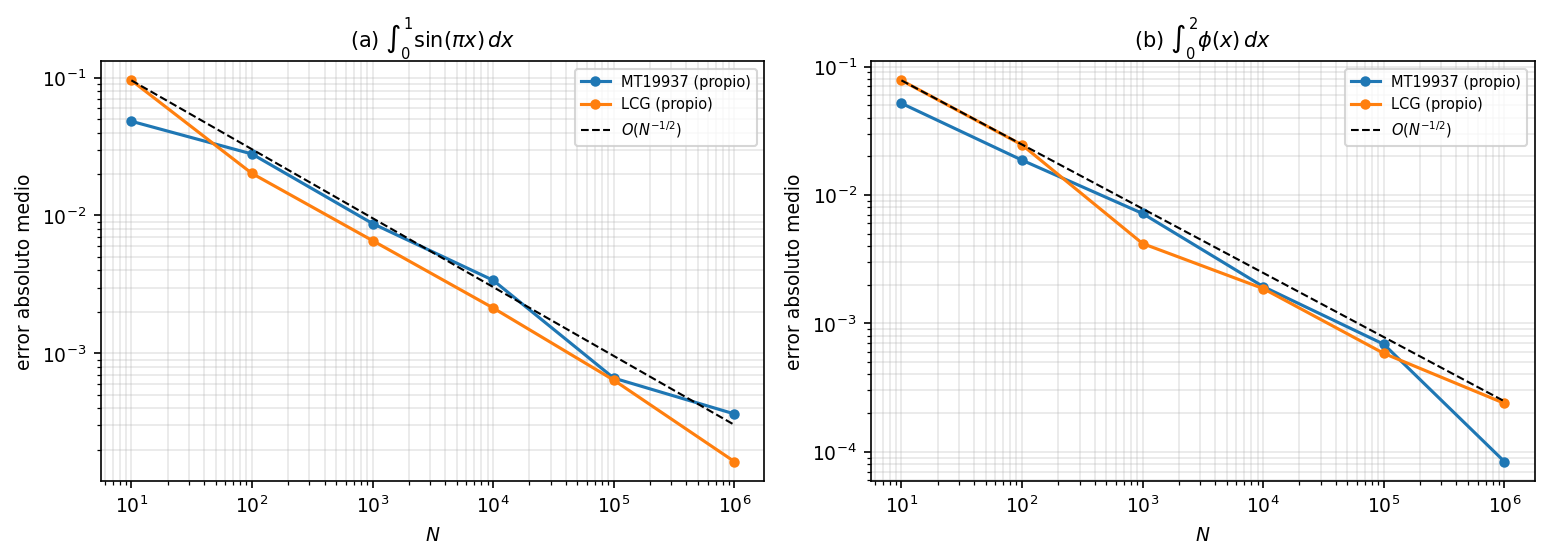
\includegraphics[width=\textwidth]{convergencia.png}
\caption{Error absoluto medio contra $N$. La recta discontinua tiene pendiente
exacta $-1/2$.}
\label{fig:convergencia}
\end{figure}

\begin{table}[H]
\centering\small
\begin{tabular}{llrrr}
\toprule
Integral & Fuente & Pendiente ajustada & Teórica & Desvío \\
\midrule
(a) & MT19937 (propio) & -0.4546 & $-0.5$ & 0.0454 \\
(a) & LCG (propio) & -0.5378 & $-0.5$ & 0.0378 \\
(b) & MT19937 (propio) & -0.5379 & $-0.5$ & 0.0379 \\
(b) & LCG (propio) & -0.5087 & $-0.5$ & 0.0087 \\
\bottomrule
\end{tabular}

\caption{Pendientes ajustadas por mínimos cuadrados sobre los logaritmos.}
\label{tab:pendientes}
\end{table}

Si $|\hat I_N - I| \approx C N^{-1/2}$, entonces
$\log|\hat I_N - I| \approx \log C - \tfrac12 \log N$, de modo que la pendiente
en escala log--log debe ser $-1/2$. Las cuatro pendientes ajustadas quedan
entre $-0.45$ y $-0.54$, con desvíos de a lo sumo $0.046$ respecto al valor
teórico. \textbf{La tasa $O(N^{-1/2})$ derivada en el
Teorema~\ref{teo:varianza} queda confirmada empíricamente.}

Los desvíos no son un defecto del método sino ruido de estimación: el error de
una corrida es una variable aleatoria, y promediar 20 réplicas reduce esa
dispersión pero no la elimina. Con $N$ grande el número de réplicas baja (para
no agotar la memoria), lo que aumenta el ruido justo en el extremo derecho de
la recta, que es donde más pesa el ajuste.

\subsection{Verificación de la cobertura}

El intervalo \eqref{eq:ic} promete atrapar el valor real el $95\,\%$ de las
veces. Eso es comprobable. Se genera una secuencia de $10^7$ uniformes, se
parte en 1000 bloques disjuntos de $N = 10^4$, se construye un intervalo por
bloque y se cuenta cuántos contienen $2/\pi$:
\[
  \textbf{946 de 1000} = 94.6\,\% ,
  \qquad \text{esperado } 950 \pm 6.9 .
\]
El resultado cae dentro de una desviación estándar del valor nominal. Se usan
bloques disjuntos de una misma corrida, y no semillas distintas, porque en un
LCG dos semillas producen secuencias relacionadas de forma determinista; los
bloques disjuntos garantizan que ningún número se reutilice entre réplicas.

\section{Alta dimensión y la maldición de la dimensionalidad}
\label{sec:mc-alta-dimension}

Se estima el volumen de la bola unitaria en $d$ dimensiones,
$V_d = \pi^{d/2}/\Gamma(d/2+1)$, muestreando puntos uniformes en el cubo
$[-1,1]^d$ y contando la fracción que cae dentro. El valor cerrado se usa
únicamente como verdad de referencia.

Como la fracción $p$ es una proporción binomial, $\mathrm{Var}(\hat p) =
p(1-p)/N$, y el intervalo se construye sobre esa varianza multiplicada por el
volumen del cubo, $2^d$.

\begin{table}[H]
\centering\small
\begin{tabular}{rrrrcrrc}
\toprule
$d$ & Aciertos & Esperados & $\hat V_d$ & IC 95\% & $V_d$ exacto & Error rel. & Contiene \\
\midrule
2 & 157\,087 & 157079.633 & 3.141740 & [3.134543, 3.148937] & 3.141593 & 0.00\% & Sí \\
5 & 33\,075 & 32898.681 & 5.292000 & [5.239897, 5.344103] & 5.263789 & 0.54\% & Sí \\
10 & 491 & 498.079 & 2.513920 & [2.291832, 2.736008] & 2.550164 & 1.42\% & Sí \\
20 & 0 & 0.005 & 0.000000 & [0.000000, 15.728640] & 0.025807 & 100.00\% & Sí \\
\bottomrule
\end{tabular}

\caption{Estimación de $V_d$ con $N = 200\,000$ puntos.}
\label{tab:mc-bola}
\end{table}

La columna de aciertos es la que cuenta la historia. En $d=2$ caen dentro
$157\,087$ puntos de $200\,000$; en $d=10$ apenas $491$; en $d=20$,
\textbf{ninguno}. Y no es un error: el número esperado de aciertos en $d=20$ es
$0.005$, así que observar cero es el resultado más probable con diferencia.

\paragraph{El intervalo cuando no hay aciertos.} Con $\hat p = 0$ el error
estándar binomial $\sqrt{\hat p(1-\hat p)/N}$ vale cero y el intervalo
\eqref{eq:ic} colapsa a $[0,0]$, que \emph{no} contiene el valor real
$V_{20} \approx 0.0258$. La aproximación normal exige varios aciertos para ser
válida. En su lugar se usa la \emph{regla de tres}: con cero éxitos en $N$
ensayos, el límite superior del intervalo del $95\,\%$ para la proporción es
aproximadamente $3/N$, lo que da $[0,\;15.73]$. Contiene el valor real, pero es
tan ancho que no informa nada. Esa inutilidad es el diagnóstico.

\subsection{Comparación contra cuadratura determinística}

\begin{table}[H]
\centering\small
\begin{tabular}{rlrrr}
\toprule
$d$ & Puntos & Evaluaciones & $\hat V_d$ rejilla & Error rel. \\
\midrule
2 & $10^{2}$ & 100 & 3.200000 & 1.86% \\
5 & $10^{5}$ & 100\,000 & 4.884480 & 7.21% \\
10 & $10^{10}$ & 10\,000\,000\,000 & inviable & --- \\
20 & $10^{20}$ & 100\,000\,000\,000\,000\,000\,000 & inviable & --- \\
\bottomrule
\end{tabular}

\caption{Cuadratura en rejilla con $m = 10$ subdivisiones por eje.}
\label{tab:mc-rejilla}
\end{table}

Una rejilla de $m=10$ por eje necesita $10^d$ evaluaciones. En $d=2$ son 100 y
en $d=5$ son cien mil, ambas triviales. En $d=10$ son \textbf{diez mil
millones}, y en $d=20$ son $10^{20}$: más evaluaciones que segundos
transcurridos desde el Big Bang. El costo crece exponencialmente con $d$
mientras el refinamiento por eje se queda clavado en 10. \emph{Eso} es la
maldición de la dimensionalidad.

\begin{table}[H]
\centering\small
\begin{tabular}{rrrrr}
\toprule
$d$ & $m$ & Presupuesto & Error rejilla & Error MC \\
\midrule
2 & 447 & 199\,809 & 0.00% & 0.00% \\
5 & 11 & 161\,051 & 2.35% & 0.39% \\
10 & 3 & 59\,049 & 36.68% & 9.56% \\
20 & 2 & 1\,048\,576 & 100.00% & 100.00% \\
\bottomrule
\end{tabular}

\caption{Error a igual presupuesto de evaluaciones: se elige $m$ tal que
$m^d \approx 200\,000$.}
\label{tab:mc-presupuesto}
\end{table}

A igual presupuesto el cruce es nítido. En $d=2$ empatan. En $d=5$ Monte Carlo
ya gana por un factor de seis. En $d=10$ el presupuesto solo alcanza para
$m=3$ subdivisiones por eje, y la rejilla se equivoca por un $36.7\,\%$ contra
el $9.6\,\%$ de Monte Carlo. La rejilla no falla por ser mala regla, sino
porque en alta dimensión el presupuesto no da ni para tres puntos por eje.

\subsection{Por qué el muestreo uniforme se vuelve ineficiente}

\begin{figure}[H]
\centering
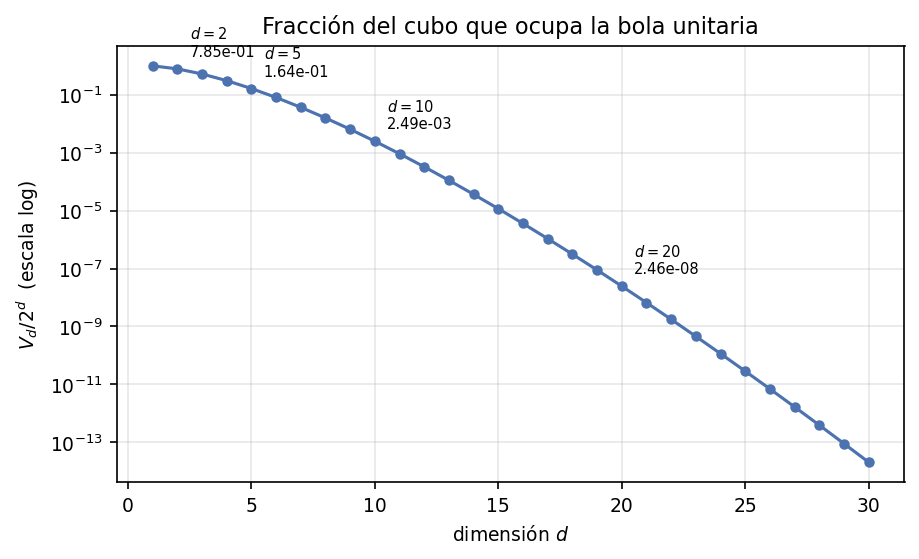
\includegraphics[width=0.75\textwidth]{fraccion_volumen.png}
\caption{Fracción del cubo $[-1,1]^d$ ocupada por la bola unitaria, en escala
logarítmica.}
\label{fig:fraccion}
\end{figure}

La fracción $V_d/2^d$ se desploma: $0.785$ en $d=2$, $0.165$ en $d=5$,
$2.5\times10^{-3}$ en $d=10$, $2.5\times10^{-8}$ en $d=20$ y
$2.0\times10^{-14}$ en $d=30$.

El fenómeno geométrico es que \textbf{en alta dimensión, casi todo el volumen
de un cubo está en sus esquinas}. La bola inscrita toca cada cara a distancia
1 del centro, pero los vértices del cubo están a distancia $\sqrt{d}$, que
crece sin límite. El cubo se vuelve, en esencia, $2^d$ púas delgadas alrededor
de una bola comparativamente diminuta.

Esto no contradice la tasa $O(N^{-1/2})$: la tasa sigue siendo $N^{-1/2}$, pero
la \emph{constante} explota. Con $p$ minúsculo, el error relativo del estimador
de proporción es
\[
  \frac{\mathrm{EE}(\hat p)}{p} = \sqrt{\frac{1-p}{Np}} \approx \frac{1}{\sqrt{Np}},
\]
así que mantener un error relativo fijo exige $N \propto 1/p = 2^d/V_d$, que en
$d=20$ significa del orden de $10^8$ puntos para un solo dígito de precisión.

La lección de diseño es que el muestreo uniforme en el cubo es la elección
equivocada: gasta prácticamente todas sus muestras en una región que no aporta.
Un buen estimador en alta dimensión debe concentrar el muestreo donde el
integrando no se anula, que es la idea del muestreo por importancia.

\section{Reducción de varianza}
\label{sec:mc-varianza}

Como el error es $\sigma/\sqrt{N}$, bajarlo admite dos caminos: subir $N$, que
cuesta tiempo lineal, o bajar $\sigma$. Se implementan dos técnicas y se
aplican a \emph{ambas} integrales de la Sección~\ref{sec:mc-integrales}, porque
el contraste entre ellas es el resultado más interesante.

\subsection{Variables antitéticas}

A cada $U$ se le empareja su reflejo $a+b-U$, que tiene la misma distribución.
Con $N/2$ uniformes se producen $N$ evaluaciones, de modo que el presupuesto se
mantiene. Escribiendo $Y = f(U)$ e $Y' = f(a+b-U)$,
\begin{equation}
  \mathrm{Var}\!\left(\frac{Y+Y'}{2}\right)
  = \frac{\mathrm{Var}(Y) + \mathrm{Var}(Y') + 2\,\mathrm{Cov}(Y,Y')}{4}
  = \frac{\mathrm{Var}(Y)\,\bigl(1 + \rho\bigr)}{2},
  \label{eq:antiteticas}
\end{equation}
donde $\rho$ es la correlación entre $Y$ e $Y'$. La técnica ayuda si y solo si
$\rho < 0$, lo que ocurre cuando $f$ es monótona: si $U$ es grande, $a+b-U$ es
pequeño, y una $f$ monótona convierte eso en valores opuestos que se compensan.

\subsection{Variables de control}

Se usa una variable $g(X)$ de media conocida $\mu_g$ y se corrige:
$Y_c = Y - c\,(g(X) - \mu_g)$. Como $\mathbb{E}[g(X)-\mu_g] = 0$, el estimador
sigue siendo insesgado para cualquier $c$. Su varianza es
\[
  \mathrm{Var}(Y_c) = \mathrm{Var}(Y) - 2c\,\mathrm{Cov}(Y,g) + c^2\mathrm{Var}(g),
\]
una parábola en $c$ cuyo mínimo está en
$c^\star = \mathrm{Cov}(Y,g)/\mathrm{Var}(g)$. Sustituyendo,
\begin{equation}
  \mathrm{Var}(Y_{c^\star}) = \mathrm{Var}(Y)\,(1-\rho^2)
  \quad\Longrightarrow\quad
  \text{factor de reducción} = \frac{1}{1-\rho^2},
  \label{eq:control}
\end{equation}
con $\rho$ la correlación entre $f$ y $g$. La técnica vale exactamente lo que
$g$ se parezca a $f$.

\subsection{Resultados}

\begin{table}[H]
\centering\small
\begin{tabular}{llrrrrc}
\toprule
Integral & Técnica & $\hat I$ & Varianza & Factor & \emph{Speedup} & IC 95\% \\
\midrule
(a) & Simple & 0.637478 & 9.4568e-02 & 1.00 & 1.00 & [0.636130, 0.638825] \\
(a) & Antitéticas & 0.637372 & 9.4585e-02 & 0.50 & 0.50 & [0.635466, 0.639279] \\
(a) & Control $g(x)=x$ & 0.637482 & 9.4566e-02 & 1.00 & 1.00 & [0.636135, 0.638830] \\
(a) & Control $g(x)=x(1-x)$ & 0.636617 & 2.9781e-04 & 317.54 & 317.54 & [0.636542, 0.636693] \\
(b) & Simple & 0.478216 & 5.2886e-02 & 1.00 & 1.00 & [0.477208, 0.479224] \\
(b) & Antitéticas & 0.477270 & 7.2851e-05 & 362.97 & 362.97 & [0.477217, 0.477323] \\
(b) & Control $g(x)=x$ & 0.477273 & 4.9911e-04 & 105.96 & 105.96 & [0.477175, 0.477371] \\
(b) & Control $g(x)=x(1-x)$ & 0.477190 & 9.9949e-03 & 5.29 & 5.29 & [0.476752, 0.477628] \\
\bottomrule
\end{tabular}

\caption{Factores de reducción con $N = 200\,000$ evaluaciones en todos los
casos.}
\label{tab:mc-varianza}
\end{table}

\paragraph{¿La técnica siempre ayuda?} No, y las dos integrales lo demuestran
en direcciones opuestas.

\emph{Antitéticas.} En la integral (b), donde $\phi$ es monótona decreciente en
$[0,2]$, el factor es $\mathbf{363\times}$. En la integral (a) el factor es
$\mathbf{0.50\times}$: la técnica \textbf{empeora} el estimador. La razón es
exacta y no estadística: $\sin(\pi(1-x)) = \sin(\pi x)$, de modo que
$Y' = Y$ idénticamente, $\rho = +1$, y \eqref{eq:antiteticas} da
$\mathrm{Var}(Y)$, la misma varianza que Monte Carlo simple, pero habiendo
gastado dos evaluaciones por muestra en lugar de una. La simetría del
integrando respecto al centro del intervalo es precisamente el peor caso.

\emph{Variables de control.} En la integral (a), el control lineal $g(x)=x$ da
$\rho = 0.004$ y un factor de $1.00\times$: no hace nada. Otra vez la simetría
es la culpable, ahora porque $\mathrm{Cov}(\sin(\pi U), U) = 0$ para
$U\sim\mathrm{Unif}(0,1)$. Basta cambiar a un control que comparta la simetría,
$g(x) = x(1-x)$, para obtener $\rho = 0.9984$ y un factor de
$\mathbf{317\times}$. En la integral (b) el orden se invierte: el control
lineal da $106\times$ y el cuadrático solo $5.3\times$.

\paragraph{Contraste con la predicción teórica.} La fórmula \eqref{eq:control}
predice un factor $1/(1-\rho^2)$. Con $\rho = 0.9984$ predice $313$ y se midió
$\mathbf{317}$; con $\rho = -0.9953$ predice $107$ y se midió $\mathbf{106}$.
La coincidencia confirma la derivación.

\paragraph{\emph{Speedup} efectivo.} Como la varianza del promedio es
inversamente proporcional a $N$, reducir la varianza por un factor $k$ equivale
a multiplicar el número de muestras por $k$. El control $g(x)=x(1-x)$ en la
integral (a) rinde como $317 \times 200\,000 \approx 6.3\times 10^{7}$ muestras
de Monte Carlo simple, a costo de una sola evaluación extra por punto.

\section{Cuando el generador arruina el resultado: RANDU}
\label{sec:mc-randu}

Se estima la integral triple
\[
  I = \iiint_{[0,1]^3} \mathbf{1}\bigl[x^2+y^2+z^2 \le 1\bigr]\,dx\,dy\,dz
  = \frac{\pi}{6} \approx 0.52359878,
\]
que depende genuinamente de ternas $(x,y,z)$, usando ternas consecutivas y
disjuntas de cada generador.

\begin{table}[H]
\centering\small
\begin{tabular}{lrcrrc}
\toprule
Fuente & $\hat I$ & IC 95\% & Error & $|$error$|/$EE & Contiene $\pi/6$ \\
\midrule
RANDU & 0.523535 & [0.522843, 0.524227] & -6.38e-05 & 0.2 & Sí \\
Mersenne Twister & 0.523711 & [0.523019, 0.524404] & +1.13e-04 & 0.3 & Sí \\
LCG (Num. Recipes) & 0.522999 & [0.522307, 0.523691] & -6.00e-04 & 1.7 & Sí \\
\bottomrule
\end{tabular}

\caption{Integral triple con $2\,000\,000$ de ternas.}
\label{tab:mc-randu}
\end{table}

\paragraph{Un resultado contrario a la expectativa.} RANDU \textbf{no falla}.
Su error es de $0.2$ errores estándar, mejor incluso que el del LCG de
Numerical Recipes ($1.7$). Los tres intervalos contienen $\pi/6$.

Esto merece explicación en vez de disimulo. Los 15 planos derivados en el
Teorema~\ref{teo:red} tienen normal $\mathbf{h}=(9,-6,1)$ y están separados por
\[
  \frac{1}{\|\mathbf{h}\|} = \frac{1}{\sqrt{81+36+1}} = \frac{1}{\sqrt{118}}
  \approx 0.0921 .
\]
La bola unitaria restringida a $[0,1]^3$ mide del orden de 1 en cada dirección,
así que la atraviesan una docena de planos. Repartir los puntos sobre planos
equiespaciados que cortan la región muchas veces se parece mucho a un muestreo
\emph{estratificado}, y la estratificación no sesga: si acaso, reduce varianza.
El defecto de RANDU no desaparece, simplemente no muerde a esta escala.

\subsection{Dónde sí muerde}

Si la estructura tiene una escala característica de $0.0921$, el fallo debe
aparecer al estimar regiones de ese tamaño o menores. Se repite el
experimento con bolas centradas en $(\tfrac12,\tfrac12,\tfrac12)$ de radio
decreciente.

\begin{table}[H]
\centering\small
\begin{tabular}{rrrrrr}
\toprule
$r$ & $V$ real & RANDU & Error & Mersenne Twister & Error \\
\midrule
0.30 & 1.131e-01 & 1.140e-01 & 0.8% & 1.132e-01 & 0.1% \\
0.15 & 1.414e-02 & 1.480e-02 & 4.7% & 1.422e-02 & 0.6% \\
0.08 & 2.145e-03 & 1.859e-03 & 13.3% & 2.238e-03 & 4.4% \\
0.05 & 5.236e-04 & 7.330e-04 & 40.0% & 5.550e-04 & 6.0% \\
0.03 & 1.131e-04 & 2.750e-04 & 143.2% & 1.260e-04 & 11.4% \\
\bottomrule
\end{tabular}

\caption{Volumen de bolas pequeñas, $10^6$ ternas. El espaciado entre planos
de RANDU es $0.0921$.}
\label{tab:randu-escala}
\end{table}

\begin{figure}[H]
\centering
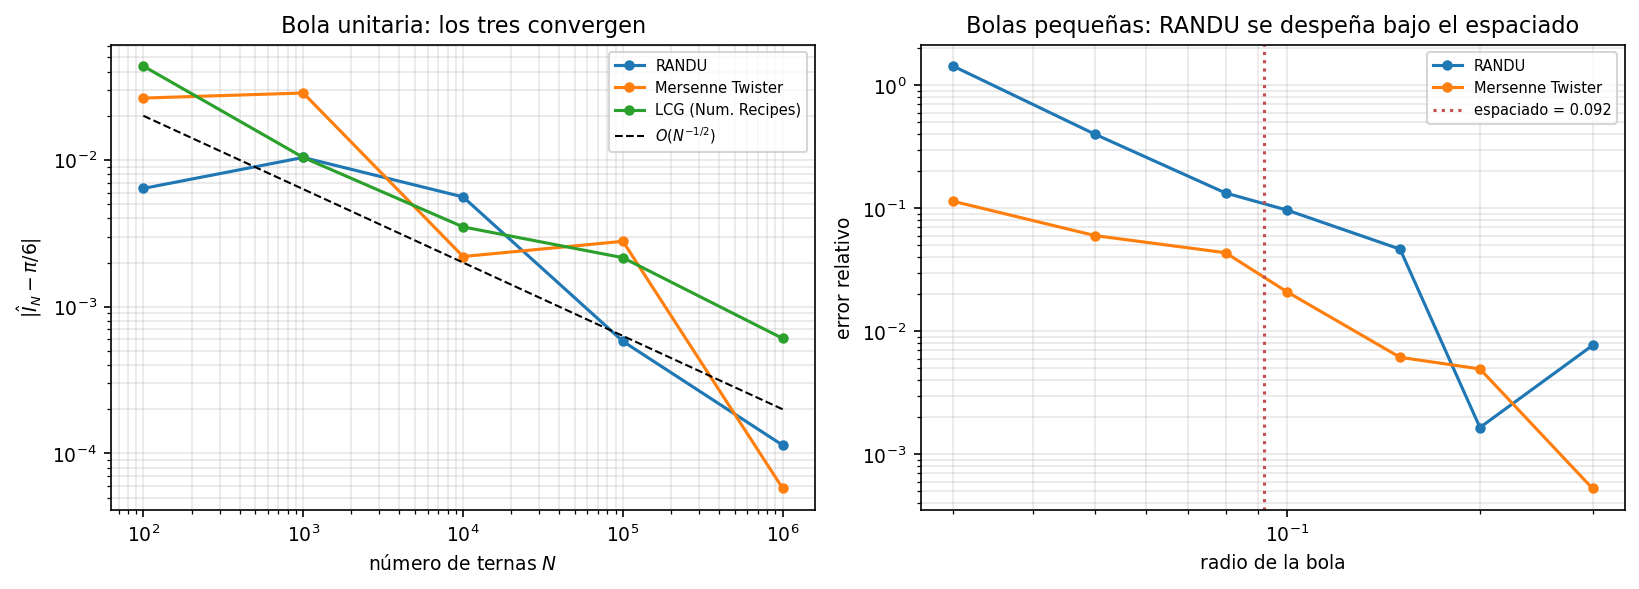
\includegraphics[width=\textwidth]{randu_convergencia.png}
\caption{Izquierda: los tres generadores convergen para la bola unitaria.
Derecha: al bajar el radio por debajo del espaciado entre planos (línea
punteada), RANDU se despeña mientras Mersenne solo acusa el ruido estadístico
de tener menos aciertos.}
\label{fig:randu-convergencia}
\end{figure}

El error de RANDU pasa de $0.8\,\%$ con radio $0.30$ a $\mathbf{143\,\%}$ con
radio $0.03$, mientras Mersenne Twister solo se degrada de $0.1\,\%$ a
$11.4\,\%$ por el ruido esperable de tener pocos aciertos. El cruce ocurre
alrededor del radio $0.05$, es decir cuando el diámetro de la bola es
comparable al espaciado entre planos.

\paragraph{La explicación geométrica.} Una bola de radio $0.03$ tiene diámetro
$0.06$, menor que la separación $0.0921$ entre planos consecutivos. Según dónde
caiga, o bien ningún plano la atraviesa —y RANDU no puede colocar un solo punto
dentro, estimando volumen cero— o bien un plano la corta por el medio y todos
los puntos de RANDU en esa zona se concentran en un disco, sobrestimando. No
hay término medio, porque \textbf{RANDU no tiene puntos entre los planos}. El
$143\,\%$ de error de la tabla es este segundo caso.

\paragraph{Conexión con la prueba espectral.} Esto es la
Sección~\ref{sec:espectral} vista desde Monte Carlo. Allí se comprobó que
$k_i = 9u_i - 6u_{i+1} + u_{i+2}$ toma exactamente 15 valores enteros, con
desviación $0.00$ respecto al entero más cercano en las $19\,998$ ternas
examinadas. Aquí se mide el precio de esa estructura: el estimador falla cuando
la región de interés es más fina que la retícula. La prueba espectral
\emph{predice} la escala a la que el estimador va a fallar, y la predicción se
cumple.

\paragraph{La moraleja, con un matiz.} Un método de Monte Carlo nunca será
mejor que su fuente de aleatoriedad. Pero el experimento obliga a precisar la
frase: la calidad de un generador no es un número único, sino que depende de la
escala a la que se lo interrogue. RANDU es perfectamente utilizable para
estimar el volumen de la bola unitaria y catastrófico para una bola de radio
$0.03$, con los mismos puntos y en el mismo cubo. Lo peligroso no es que un
generador sea malo: es que sea malo \emph{solo} en el régimen que uno necesita,
mientras pasa todas las pruebas que uno corre.


\begin{thebibliography}{9}

\bibitem{hulldobell}
  T.~E. Hull y A.~R. Dobell. ``Random Number Generators''.
  \emph{SIAM Review} 4.3 (1962), pp.~230--254.
  doi: 10.1137/1004061.

\bibitem{marsaglia}
  G. Marsaglia. ``Random Numbers Fall Mainly in the Planes''.
  \emph{Proceedings of the National Academy of Sciences} 61.1 (1968),
  pp.~25--28. doi: 10.1073/pnas.61.1.25.

\bibitem{knuth}
  D.~E. Knuth. \emph{The Art of Computer Programming, Vol. 2:
  Seminumerical Algorithms}. 3.\textsuperscript{a} ed. Addison-Wesley, 1997.
  Capítulo 3.

\bibitem{vonneumann}
  J. von Neumann. ``Various Techniques Used in Connection with Random Digits''.
  \emph{National Bureau of Standards Applied Mathematics Series} 12 (1951),
  pp.~36--38.

\bibitem{matsumoto}
  M. Matsumoto y T. Nishimura. ``Mersenne Twister: A 623-Dimensionally
  Equidistributed Uniform Pseudo-Random Number Generator''.
  \emph{ACM Transactions on Modeling and Computer Simulation} 8.1 (1998),
  pp.~3--30. doi: 10.1145/272991.272995.

\bibitem{bbs}
  L. Blum, M. Blum y M. Shub. ``A Simple Unpredictable Pseudo-Random Number
  Generator''. \emph{SIAM Journal on Computing} 15.2 (1986), pp.~364--383.
  doi: 10.1137/0215025.

\bibitem{law}
  A.~M. Law. \emph{Simulation Modeling and Analysis}. 5.\textsuperscript{a} ed.
  McGraw-Hill, 2015.

\bibitem{randomorg}
  RANDOM.ORG. \emph{Introduction to Randomness and Random Numbers}.
  \url{https://www.random.org/randomness/}.

\end{thebibliography}

\end{document}
